\documentclass[14pt]{extbook}
\usepackage{multicol, enumerate, enumitem, hyperref, color, soul, setspace, parskip, fancyhdr} %General Packages
\usepackage{amssymb, amsthm, amsmath, bbm, latexsym, units, mathtools} %Math Packages
\everymath{\displaystyle} %All math in Display Style
% Packages with additional options
\usepackage[headsep=0.5cm,headheight=12pt, left=1 in,right= 1 in,top= 1 in,bottom= 1 in]{geometry}
\usepackage[usenames,dvipsnames]{xcolor}
\usepackage{dashrule}  % Package to use the command below to create lines between items
\newcommand{\litem}[1]{\item#1\hspace*{-1cm}\rule{\textwidth}{0.4pt}}
\pagestyle{fancy}
\lhead{Makeup Progress Quiz 1}
\chead{}
\rhead{Version C}
\lfoot{6018-3080}
\cfoot{}
\rfoot{Spring 2021}
\begin{document}

\begin{enumerate}
\litem{
Graph the equation below.\[ f(x) = -(x+1)^2 + 16 \]\begin{enumerate}[label=\Alph*.]
\begin{multicols}{2}\item 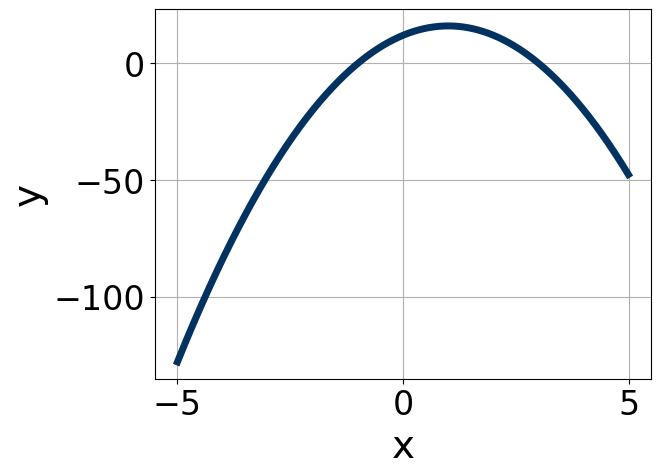
\includegraphics[width = 0.3\textwidth]{../Figures/quadraticEquationToGraphAC.png}\item 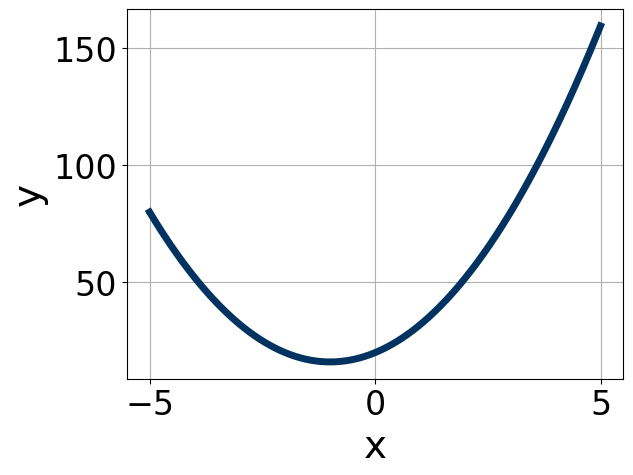
\includegraphics[width = 0.3\textwidth]{../Figures/quadraticEquationToGraphBC.png}\item 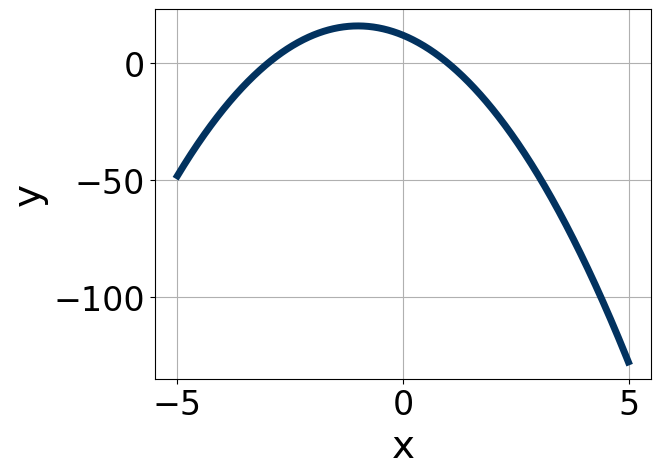
\includegraphics[width = 0.3\textwidth]{../Figures/quadraticEquationToGraphCC.png}\item 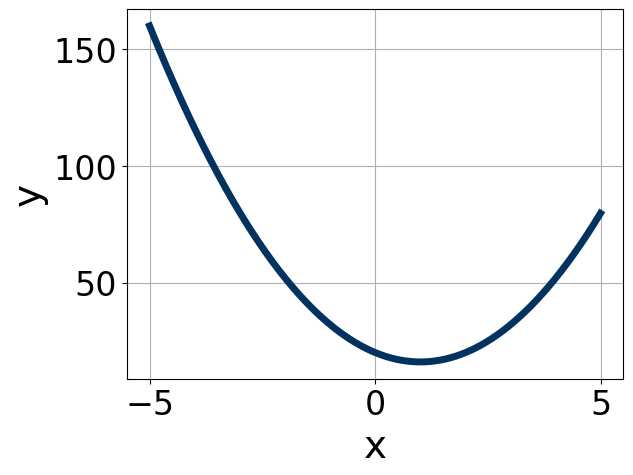
\includegraphics[width = 0.3\textwidth]{../Figures/quadraticEquationToGraphDC.png}\end{multicols}\item None of the above.
\end{enumerate} }
\litem{
Write the equation of the graph presented below in the form $f(x)=ax^2+bx+c$, assuming  $a=1$ or $a=-1$. Then, choose the intervals that $a, b,$ and $c$ belong to.
\begin{center}
    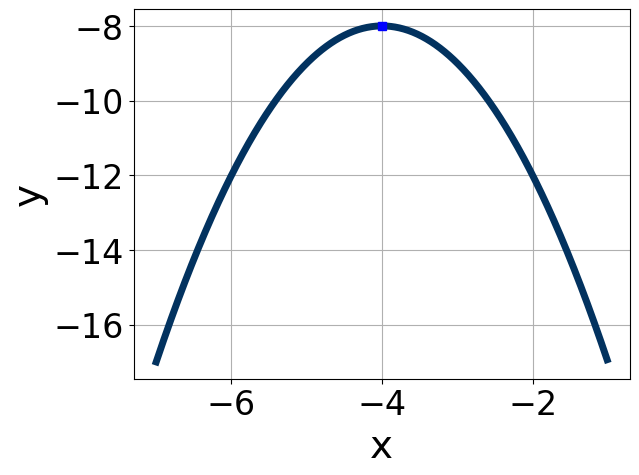
\includegraphics[width=0.5\textwidth]{../Figures/quadraticGraphToEquationCopyC.png}
\end{center}
\begin{enumerate}[label=\Alph*.]
\item \( a \in [0, 5], \hspace*{5mm} b \in [-9, -7], \text{ and } \hspace*{5mm} c \in [8, 12] \)
\item \( a \in [-6, 0], \hspace*{5mm} b \in [8, 10], \text{ and } \hspace*{5mm} c \in [-10, -7] \)
\item \( a \in [-6, 0], \hspace*{5mm} b \in [-9, -7], \text{ and } \hspace*{5mm} c \in [-24, -22] \)
\item \( a \in [0, 5], \hspace*{5mm} b \in [8, 10], \text{ and } \hspace*{5mm} c \in [8, 12] \)
\item \( a \in [-6, 0], \hspace*{5mm} b \in [8, 10], \text{ and } \hspace*{5mm} c \in [-24, -22] \)

\end{enumerate} }
\litem{
Solve the quadratic equation below. Then, choose the intervals that the solutions belong to, with $x_1 \leq x_2$ (if they exist).\[ 16x^{2} +8 x -2 = 0 \]\begin{enumerate}[label=\Alph*.]
\item \( x_1 \in [-0.89, -0.6] \text{ and } x_2 \in [-0.37, 0.21] \)
\item \( x_1 \in [-12.13, -10.02] \text{ and } x_2 \in [2.26, 3.39] \)
\item \( x_1 \in [-14.59, -14.02] \text{ and } x_2 \in [13.27, 14.07] \)
\item \( x_1 \in [-0.44, 0.68] \text{ and } x_2 \in [0.6, 0.86] \)
\item \( \text{There are no Real solutions.} \)

\end{enumerate} }
\litem{
Write the equation of the graph presented below in the form $f(x)=ax^2+bx+c$, assuming  $a=1$ or $a=-1$. Then, choose the intervals that $a, b,$ and $c$ belong to.
\begin{center}
    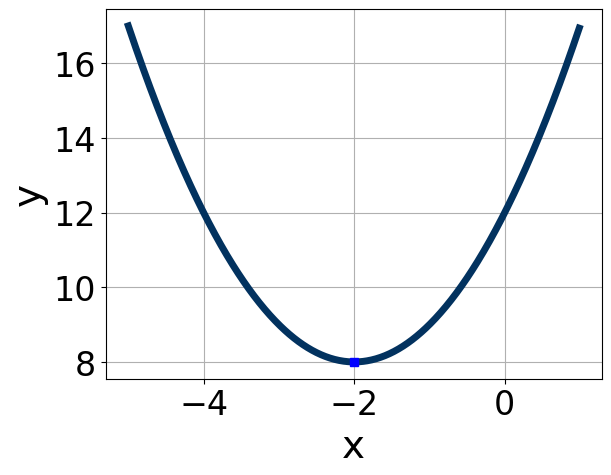
\includegraphics[width=0.5\textwidth]{../Figures/quadraticGraphToEquationC.png}
\end{center}
\begin{enumerate}[label=\Alph*.]
\item \( a \in [-0.1, 3], \hspace*{5mm} b \in [3, 8], \text{ and } \hspace*{5mm} c \in [11, 14] \)
\item \( a \in [-1.7, -0.5], \hspace*{5mm} b \in [-9, -3], \text{ and } \hspace*{5mm} c \in [4, 9] \)
\item \( a \in [-0.1, 3], \hspace*{5mm} b \in [-9, -3], \text{ and } \hspace*{5mm} c \in [-5, -1] \)
\item \( a \in [-1.7, -0.5], \hspace*{5mm} b \in [3, 8], \text{ and } \hspace*{5mm} c \in [4, 9] \)
\item \( a \in [-0.1, 3], \hspace*{5mm} b \in [-9, -3], \text{ and } \hspace*{5mm} c \in [11, 14] \)

\end{enumerate} }
\litem{
Solve the quadratic equation below. Then, choose the intervals that the solutions $x_1$ and $x_2$ belong to, with $x_1 \leq x_2$.\[ 15x^{2} +38 x + 24 = 0 \]\begin{enumerate}[label=\Alph*.]
\item \( x_1 \in [-20.24, -19.6] \text{ and } x_2 \in [-18.01, -17.97] \)
\item \( x_1 \in [-1.65, -1.2] \text{ and } x_2 \in [-1.24, -1.08] \)
\item \( x_1 \in [-3.15, -2.58] \text{ and } x_2 \in [-0.62, -0.58] \)
\item \( x_1 \in [-2.42, -1.89] \text{ and } x_2 \in [-0.71, -0.66] \)
\item \( x_1 \in [-6.01, -5.65] \text{ and } x_2 \in [-0.27, -0.22] \)

\end{enumerate} }
\litem{
Graph the equation below.\[ f(x) = (x+3)^2 + 20 \]\begin{enumerate}[label=\Alph*.]
\begin{multicols}{2}\item 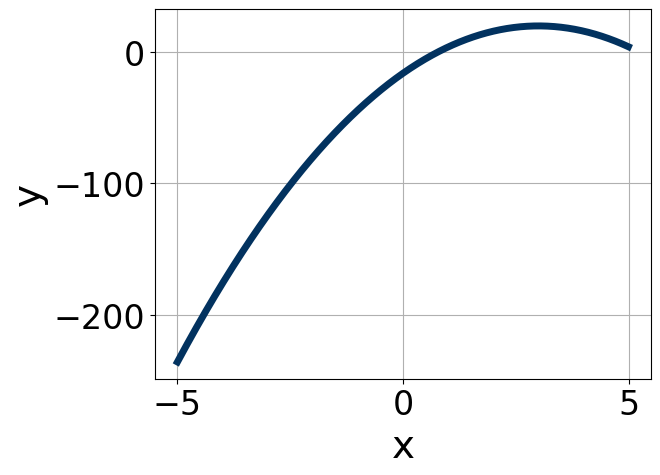
\includegraphics[width = 0.3\textwidth]{../Figures/quadraticEquationToGraphCopyAC.png}\item 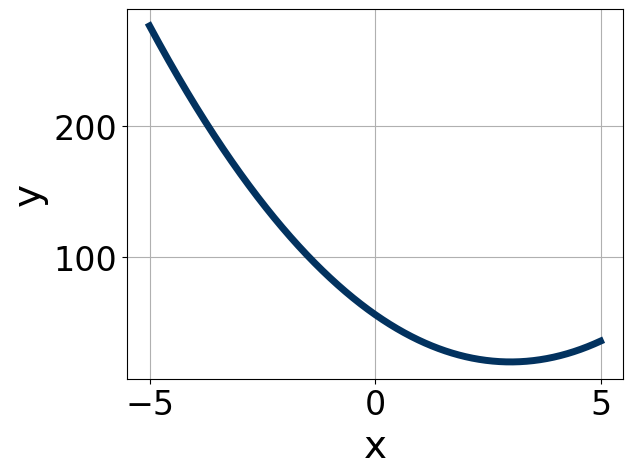
\includegraphics[width = 0.3\textwidth]{../Figures/quadraticEquationToGraphCopyBC.png}\item 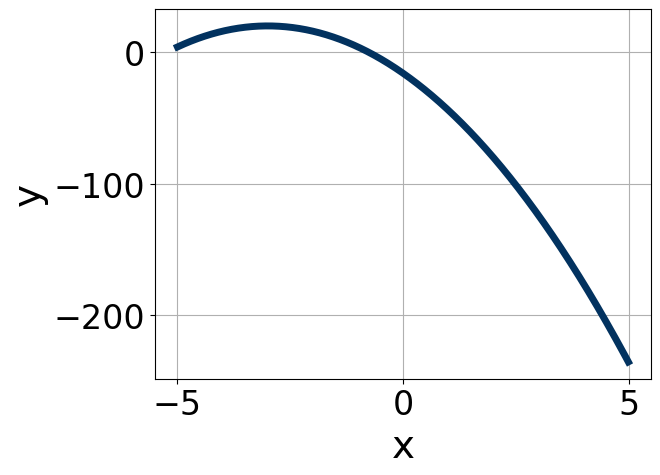
\includegraphics[width = 0.3\textwidth]{../Figures/quadraticEquationToGraphCopyCC.png}\item 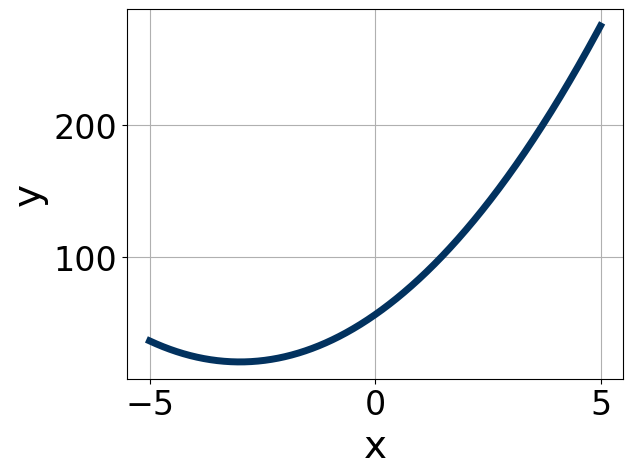
\includegraphics[width = 0.3\textwidth]{../Figures/quadraticEquationToGraphCopyDC.png}\end{multicols}\item None of the above.
\end{enumerate} }
\litem{
Factor the quadratic below. Then, choose the intervals that contain the constants in the form $(ax+b)(cx+d); b \leq d.$\[ 36x^{2} -60 x + 25 \]\begin{enumerate}[label=\Alph*.]
\item \( a \in [-0.51, 2.66], \hspace*{5mm} b \in [-31, -25], \hspace*{5mm} c \in [-2, 2], \text{ and } \hspace*{5mm} d \in [-33, -25] \)
\item \( a \in [1.97, 3.52], \hspace*{5mm} b \in [-8, -3], \hspace*{5mm} c \in [12, 16], \text{ and } \hspace*{5mm} d \in [-8, 1] \)
\item \( a \in [5.91, 6.33], \hspace*{5mm} b \in [-8, -3], \hspace*{5mm} c \in [6, 11], \text{ and } \hspace*{5mm} d \in [-8, 1] \)
\item \( a \in [11.13, 12.66], \hspace*{5mm} b \in [-8, -3], \hspace*{5mm} c \in [2, 5], \text{ and } \hspace*{5mm} d \in [-8, 1] \)
\item \( \text{None of the above.} \)

\end{enumerate} }
\litem{
Solve the quadratic equation below. Then, choose the intervals that the solutions $x_1$ and $x_2$ belong to, with $x_1 \leq x_2$.\[ 10x^{2} -57 x + 54 = 0 \]\begin{enumerate}[label=\Alph*.]
\item \( x_1 \in [0.87, 1.19] \text{ and } x_2 \in [6, 9] \)
\item \( x_1 \in [11.39, 12.23] \text{ and } x_2 \in [43, 46] \)
\item \( x_1 \in [1.08, 1.5] \text{ and } x_2 \in [3.5, 5.5] \)
\item \( x_1 \in [0.28, 0.53] \text{ and } x_2 \in [9.5, 20.5] \)
\item \( x_1 \in [2.2, 2.58] \text{ and } x_2 \in [-0.6, 4.4] \)

\end{enumerate} }
\litem{
Solve the quadratic equation below. Then, choose the intervals that the solutions belong to, with $x_1 \leq x_2$ (if they exist).\[ 12x^{2} -10 x -6 = 0 \]\begin{enumerate}[label=\Alph*.]
\item \( x_1 \in [-19.6, -17.8] \text{ and } x_2 \in [19, 20.8] \)
\item \( x_1 \in [-0.8, 0.4] \text{ and } x_2 \in [0.9, 1.7] \)
\item \( x_1 \in [-5.6, -3.9] \text{ and } x_2 \in [14.7, 15.1] \)
\item \( x_1 \in [-4, -0.5] \text{ and } x_2 \in [-0.9, 1.2] \)
\item \( \text{There are no Real solutions.} \)

\end{enumerate} }
\litem{
Factor the quadratic below. Then, choose the intervals that contain the constants in the form $(ax+b)(cx+d); b \leq d.$\[ 24x^{2} -38 x + 15 \]\begin{enumerate}[label=\Alph*.]
\item \( a \in [2.55, 3.75], \hspace*{5mm} b \in [-8, 0], \hspace*{5mm} c \in [7.41, 8.02], \text{ and } \hspace*{5mm} d \in [-6, 5] \)
\item \( a \in [10.91, 13.92], \hspace*{5mm} b \in [-8, 0], \hspace*{5mm} c \in [1.81, 2.98], \text{ and } \hspace*{5mm} d \in [-6, 5] \)
\item \( a \in [-1.1, 2.34], \hspace*{5mm} b \in [-21, -18], \hspace*{5mm} c \in [0.03, 1.59], \text{ and } \hspace*{5mm} d \in [-21, -15] \)
\item \( a \in [4.44, 8.38], \hspace*{5mm} b \in [-8, 0], \hspace*{5mm} c \in [3.65, 5.66], \text{ and } \hspace*{5mm} d \in [-6, 5] \)
\item \( \text{None of the above.} \)

\end{enumerate} }
\end{enumerate}

\end{document}